\documentclass[conference]{IEEEtran}


  	\usepackage[pdftex]{graphicx}
  	\graphicspath{{../pdf/}{../jpeg/}}
	\DeclareGraphicsExtensions{.pdf,.jpeg,.png}

	\usepackage[cmex10]{amsmath}
	\usepackage{mathabx}
	\usepackage{algorithmic}
	\usepackage{array}
	\usepackage{mdwmath}
	\usepackage{mdwtab}
	\usepackage{eqparbox}
	\usepackage{url}
	\hyphenation{op-tical net-works semi-conduc-tor}



\begin{document}

\title{\LARGE Design and Analysis of Algorithms Assignment- 4
}


 \author{\authorblockN{Harsha Vardhan Madasi(IIT2019108), \,Rahul Kumar(IIT2019109),\, Sumit Katiyar(IIT2019029)\\.}
 }
 
 \author{ \IEEEauthorblockN{Harsha Vardhan Madasi-IIT2019108}
\IEEEauthorblockN{Rahul Kumar-IIT2019109}
\IEEEauthorblockN{Sumit Katiyar-IIT2019110}
\authorblockA{B.Tech. 4th semester, Department of Information Technology}\\
\authorblockA{Indian Institute of Information Technology, Allahabad}
}


\maketitle

\begin{abstract}
\textit{ Given an array of 2n elements in the following format { a1, a2, a3, a4,
....., an, b1, b2, b3, b4, ...., bn }. The task is shuffle the array to {a1, b1,
a2, b2, a3, b3, ......, an, bn } without using extra space.}
\end{abstract}

\IEEEoverridecommandlockouts


\IEEEpeerreviewmaketitle

% INTRODUCTION 

\section{\textbf{ INTRODUCTION}}
In this problem, we have to shuffle a given array in such a way that if the given array is a1, a2, a3, a4....., an, b1, b2, b3, b4, ...., bn. The task is shuffle the array to {a1, b1,a2, b2, a3, b3, ......, an, bn }using divide and conquer algorithm.\\\\
Divide and Conquer Algorithm:
This technique can be divided into the following three parts:
\begin{itemize}
  \item \textbf{Divide:} This involves dividing the problem into some sub problem.
  \item \textbf{Conquer:} Sub problem by calling recursively until sub problem solved.
  \item \textbf{Combine:} The Sub problem Solved so that we will get find problem solution.
\end{itemize}\\\\
This report further contains:-
\begin{enumerate}
  \item Algorithm Design
  \item Algorithm Analysis
  \item Profiling
  \item Conclusion
\end{enumerate}

% ALGORITHM DESIGN

\section{\textbf{ ALGORITHM DESIGN }}
Basically, we have come up with an approach Using divide and conquer algorithm
\hfill \break
\textbf{\underline{Algorithm: Divide and Conquer}}\\\\
In this algorithm we divide the given array into half (say arr1[] and arr2[]) and swap second half element of arr1[] with first half element of arr2[]. Recursively do this for arr1 and arr2.\\\\
\textbf{\underline{For example:}}\\
\begin{itemize}
  \item Let us consider an array be a1, a2, a3, a4, b1, b2, b3, b4.
  \item Now split the array into two halves i.e., {a1, a2, a3, a4} ;{ b1, b2, b3, b4}.
\item Now we will swap elements which are present around the center i.e., we will swap a3, a4 with b1, b2 correspondingly.
\item After swapping we will  get: a1, a2, b1, b2, a3, a4, b3, b4
\item Now we will recursively split the above subarrays and swap the elements around the center for each subarray.
\item Finally we will get a1, b1, a2, b2 and a3, b3, a4, b4.
\end{itemize}\hfill \break

% PSEUDO CODE



\textbf{\underline{PSEUDO CODE:}}\\\\
//Function to shufle an array\\
Void shuflearray(int arr[],int start , int end) \\
// base condition \\
\indent\hspace{0.5cm} if(end  \textless  start )then\\
\indent\hspace{1.0cm} return ;\\\\
//if only two elements present in the subarray\\
\indent\hspace{0.5cm} if(end  = start + 1)then\\
\indent\hspace{1.0cm} return ;\\\\
//Finding middle of the array to divide the array\\
int mid ← (start + end) /2;\\\\
//using  temp in order to swap first half of second array\\
int  temp ← mid +1;\\\\
//using  first in order to swap second half of first array\\
int firstmid ← (start + mid)/2;\\\\
//Swapping the center elements\\
for(i = firstmid +1 to i \textless = mid )\\
\indent\hspace{0.5cm}swap (arr[i],arr[temp++]);\\
\indent\hspace{0.5cm}i ← i+1;\\\\
// recursively calling the function for first and second subarrays\\
shuflearray(arr, start, mid);\\
shuflearray(arr, mid + end, l);\\\\\\\\

\textbf{//MAIN FUNCTION}\\

int main()\\
\indent\hspace{0.5cm}int n; \\
\indent\hspace{0.5cm}input  n;\\
\indent\hspace{0.5cm}int  arr[n];\\
\indent\hspace{0.5cm}//taking input\\
\indent\hspace{0.5cm}for(int i = 0 to n )\\
\indent\hspace{1.0cm}input  arr[i];\\
\indent\hspace{0.5cm}shuflearray (arr,0,n-1);\\
\indent\hspace{0.5cm}//printing the final shuffled array\\
\indent\hspace{0.5cm}for(int i = 0 to n )\\
\indent\hspace{1.0cm}print  arr[i];\\
\indent\hspace{0.5cm}return 0;\\


% ALGORITHM ANALYSIS

\section{\textbf{ALGORITHM ANALYSIS :}}
\textbf{Time complexity:}  \\
In the above algorithm we get the recurrence\\
T(n)=2T(n/2)+O(n)\\
for the time complexity, which results in \\
T(n)=O(nlogn)\\
So the final computational time to shuffle the given array is O(nlog⁡n).\\

\textbf{Space complexity:}\\
To be precise,as we are swapping the elements in the given array itself  there is no extra space required.So the space complexity will be O(1).

%  EXPERIMENTAL STUDY 

\section{\textbf{PROFILING :}}
\textbf{Posteriori Analysis}
So after the above discussion of the time and space complexity in asymptotic analysis , we come to the profiling part.

Following given is the graphical representation  of time complexity of the Algorithm  approach given below.

\begin{figure}[ht!] %!t
\centering
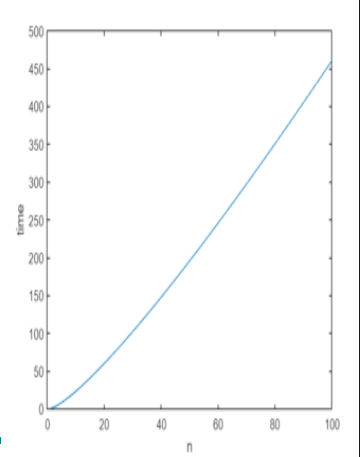
\includegraphics[width=3.5in,height=3in]{graph.png}
\caption{Time complexity graph(O(nlogn))}
\label{Courant_2}
\end{figure}\hfill \break\hfill \break


%  CONCLUSION

\section{\textbf{Conclusion}}
Hence, from the above graph and analysis, we come to the conclusion that this problem can be solved using the time complexity of O(nlogn) and space complexity of O(1). 

% REFERENCES 

\section{\textbf{References}}
\begin{enumerate}
  \item Introduction to Algorithms by Cormen,Charles,Rivest and Stein.\\
  \item Geeksfor Geeks.\\
 
\end{enumerate}
\end{document}
